\subsection{UC14 - Telegram - Autenticazione}
		
		%\begin{figure}[t!]
		%	\centering
		%	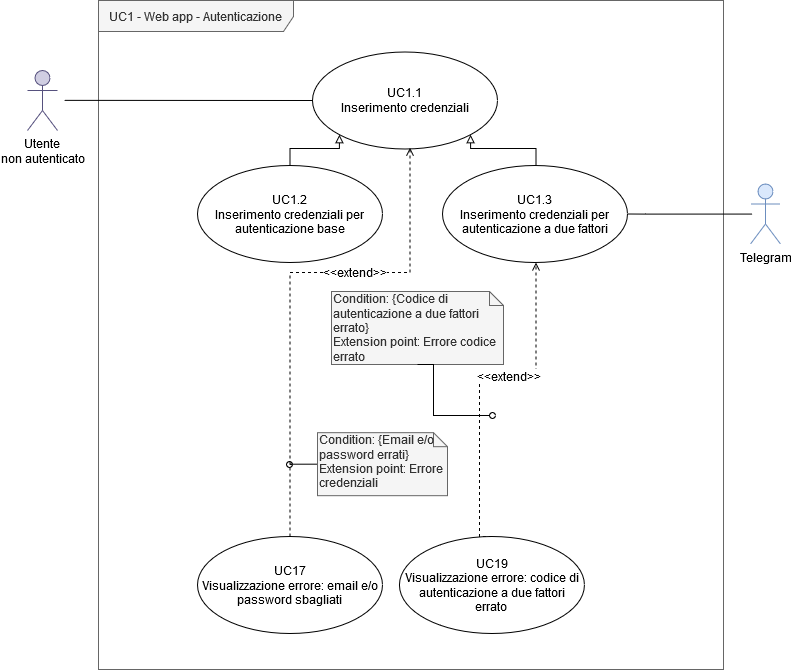
\includegraphics[height=10em]{res/images/uc1}
		%\end{figure}
		
	\begin{itemize}
		\item \textbf{Attori Primari}: Utente non autenticato.
		\item \textbf{Attori Secondari}: \glock{Telegram}.
		\item \textbf{Descrizione}: L'utente tenta di autenticarsi con il bot \glock{Telegram} entrando all'interno dell'applicazione e iniziando la chat con il bot. Attraverso \glock{Telegram}, viene segnalato al bot se l'utente che sta scrivendo ha uno username censito nel sistema. Se viene riconosciuto, viene registrata l'apertura e l'autenticazione del canale di comunicazione tra il bot e l'utente, diventando quest'ultimo autenticato. 
		\item \textbf{Precondizione}: L'utente è nell'applicazione di \glock{Telegram} e non ha una chat autenticata con il bot.
		\item \textbf{Postcondizione}: L'utente effettua l'autenticazione e il canale di comunicazione tra utente e bot viene salvato nel sistema.
		\item \textbf{Scenario Principale}:
		\begin{enumerate}
			\item L'utente seleziona nell'applicazione di \glock{Telegram} il Bot di sistema dal pannello di ricerca
			\item L'utente tenta di aprire una conversazione con il bot
			\item L'utente viene autenticato e la chat viene salvata nel sistema
		\end{enumerate}
	\end{itemize}
	
	\subsubsection{UC 14.1 - Richiesta di riconoscimento con il bot tramite /start}

	\begin{itemize}
		\item \textbf{Attori Primari}: Utente non autenticato.
		\item \textbf{Descrizione}: L'utente invia una richiesta al bot di volersi autenticare, così da aprire un canale di comunicazione.
		\item \textbf{Precondizione}: L'utente è nell'applicazione di \glock{Telegram} e non ha una chat autenticata con il bot.
		\item \textbf{Postcondizione}: L'utente effettua il riconoscimento con il sistema.
		\item \textbf{Scenario Principale}:
		\begin{enumerate}
			\item L'utente seleziona nell'applicazione di Telegram il Bot di sistema
			\item L'utente tenta di aprire una conversazione con il bot
			\item Per attivare la conversazione con il bot, viene inviato il comando predefinito /start
			\item L'utente viene autenticato e la chat viene salvata nel sistema
		\end{enumerate}
		\item \textbf{Inclusioni}:
		\begin{itemize}
			\item Controllo credenziali (UC 14.2)
		\end{itemize}
		\item \textbf{Estensioni}:
		\begin{itemize}
			\item Errore: nome utente telegram non riconosciuto (UC 14.3)
		\end{itemize}
	\end{itemize}

	\subsubsection{UC 14.2 - Controllo credenziali}

	\begin{itemize}
		\item \textbf{Attori Primari}: Utente non autenticato.
		\item \textbf{Attori Secondari}: \glock{Telegram}.
		\item \textbf{Descrizione}: Si deve verificare se il nome utente è stato gestito da parte del sistema, così da abilitare la chat di comunicazione.
		\item \textbf{Precondizione}: L'utente, tramite \glock{Telegram}, ha inviato una richiesta di avvio conversazione con il comando /start.
		\item \textbf{Postcondizione}: L'utente effettua il riconoscimento con il sistema.
		\item \textbf{Scenario Principale}:
		\begin{enumerate}
			\item \glock{Telegram} riceve in input il comando, che viene inoltrato al sistema, insieme alle informazioni relative alla chat e all'autore del messaggio.
			\item Viene mostrato un messaggio dal bot attraverso \glock{Telegram} che conferma le credenziali dell'utente con un messaggio di benvenuto.
			\item L'utente viene autenticato e la chat viene salvata nel sistema.
		\end{enumerate}
	\end{itemize}

	\subsubsection{UC 14.3 - Errore: nome utente telegram non riconosciuto}

	\begin{itemize}
		\item \textbf{Attori Primari}: Utente non autenticato.
		\item \textbf{Descrizione}: L'autenticazione della chat tra il bot e l'utente non va a buon fine dal momento che lo username associato all'account di \glock{Telegram} non è censito nel sistema.
		\item \textbf{Precondizione}: L'utente, tramite \glock{Telegram}, sta tentando di autenticarsi.
		\item \textbf{Postcondizione}: Viene mostrato un messaggio di errore che impedisce l'autenticazione della chat.
		\item \textbf{Scenario Principale}:
		\begin{enumerate}
			\item \glock{Telegram} riceve in input il comando, che viene inoltrato al sistema, insieme alle informazioni relative alla chat e all'autore del messaggio.
			\item Viene mostrato un messaggio di errore che segnala che il nome utente associato all'utente \glock{Telegram} non è censito nel sistema.
			\item L'utente non viene autenticato.
		\end{enumerate}
	\end{itemize}